\documentclass[en,black,normal,10pt]{elegantnote}
\usepackage{colortbl} % Required for colored rows
\usepackage{xcolor}
\usepackage{lipsum} % Required for generating dummy text
\usepackage{tikz}
\usepackage{caption}
\usetikzlibrary{trees,matrix,arrows,positioning}

\setlength{\parindent}{0pt}

\title{DSAA 5002 - HW1}

%\version{Fall Semester 2023}

\author{50015976 Ruiming ZHANG}
%\institute{Elegant\LaTeX{} Program}

\date{}

\usetikzlibrary{shapes,arrows}

\begin{document}

\maketitle
% logo
%\centerline{\includegraphics[width=0.2\textwidth]{logo-blue}}

\section*{Q1 [15 Marks]}

Given the transaction database below,set the minimum support count to 2 and the minimum confidence level to 60\% to find the strong association rule.
Generate the set $C_3$ of the candidate 3-itemset, using prunning on Apriori principle.

\definecolor{Gray}{gray}{0.85} % Define a custom color

\subsection*{Solution:}

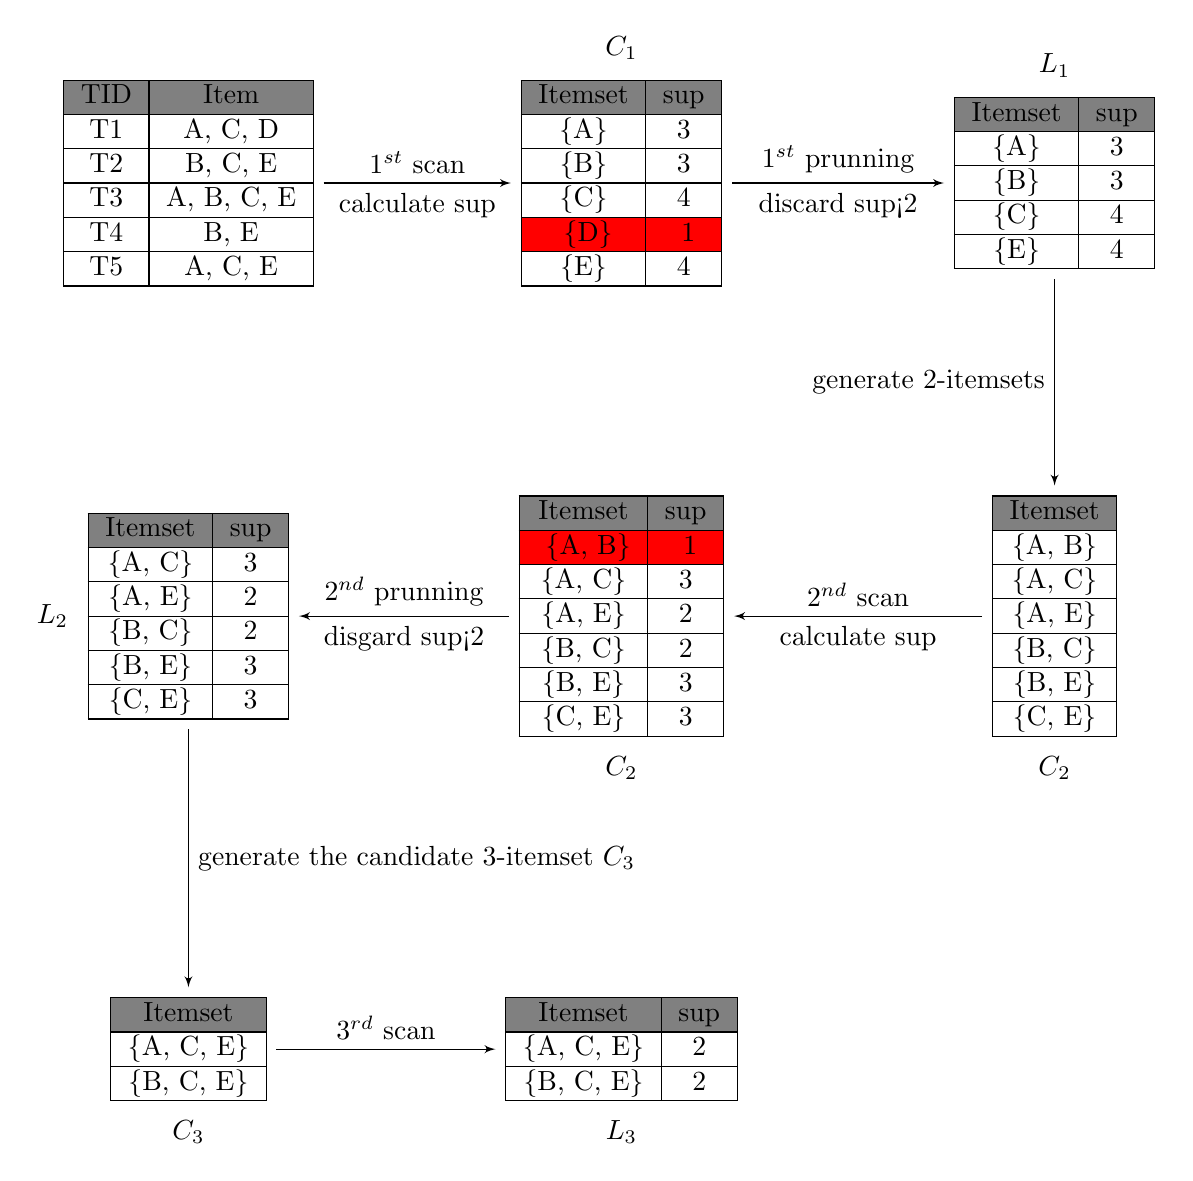
\begin{tikzpicture}[node distance = 5.5cm, auto]
    % Define block styles
    \tikzstyle{block} = [rectangle, fill=none,
                        text centered, rounded corners, minimum height=4em]
    \tikzstyle{line} = [draw, -latex']

    % Place nodes
    \node [block] (item1) {
      \begin{tabular}{|c|c|c|}
        \hline
          \rowcolor{Gray} % Set the color of the first row to gray
          TID & Item \\
          \hline
          T1 & A, C, D \\
          \hline
          T2 & B, C, E \\
          \hline
          T3 & A, B, C, E \\
          \hline
          T4 & B, E \\
          \hline
          T5 & A, C, E \\
          \hline
      \end{tabular}
    };

    \node [block, right  of=item1, label=above:$C_1$] (scan1) {
      \begin{tabular}{|c|c|c|}
        \hline
        \rowcolor{Gray} % Set the color of the first row to gray
        Itemset & sup \\
        \hline
        {\{A\}} & 3 \\
        \hline
        {\{B\}} & 3 \\
        \hline
        {\{C\}} & 4 \\
        \hline
        \cellcolor{red} {\{D\}} & \cellcolor{red} 1 \\
        \hline
        {\{E\}} & 4 \\
        \hline
      \end{tabular}
    };

    \node [block, right of=scan1, label=above:$L_1$] (prunning1) {
      \begin{tabular}{|c|c|c|}
        \hline
        \rowcolor{Gray} % Set the color of the first row to gray
        Itemset & sup \\
        \hline
        {\{A\}} & 3 \\
        \hline
        {\{B\}} & 3 \\
        \hline
        {\{C\}} & 4 \\
        \hline
        {\{E\}} & 4 \\
        \hline
      \end{tabular}
    };

    \node [block, below of=prunning1, label=below:$C_2$] (item2) {
      \begin{tabular}{|c|c|}
        \hline
        \rowcolor{Gray} % Set the color of the first row to gray
        Itemset \\
        \hline
        {\{A, B\}} \\
        \hline
        {\{A, C\}} \\
        \hline
        {\{A, E\}} \\
        \hline
        {\{B, C\}} \\
        \hline
        {\{B, E\}} \\
        \hline
        {\{C, E\}} \\
        \hline 
      \end{tabular}
    };

    \node [block, left of=item2, label=below:$C_2$] (scan2) {
      \begin{tabular}{|c|c|c|}
        \hline
        \rowcolor{Gray} % Set the color of the first row to gray
        Itemset & sup \\
        \hline
        \cellcolor{red} {\{A, B\}} & \cellcolor{red} 1 \\
        \hline
        {\{A, C\}} & 3 \\
        \hline
        {\{A, E\}} & 2 \\
        \hline
        {\{B, C\}} & 2 \\
        \hline
        {\{B, E\}} & 3 \\
        \hline
        {\{C, E\}} & 3 \\
        \hline 
      \end{tabular}
    };

    \node [block, left of=scan2, label=left:$L_2$] (prunning2) {
      \begin{tabular}{|c|c|c|}
        \hline
        \rowcolor{Gray} % Set the color of the first row to gray
        Itemset & sup \\
        \hline
        {\{A, C\}} & 3 \\
        \hline
        {\{A, E\}} & 2 \\
        \hline
        {\{B, C\}} & 2 \\
        \hline
        {\{B, E\}} & 3 \\
        \hline
        {\{C, E\}} & 3 \\
        \hline 
      \end{tabular}
    };

    \node [block, below of=prunning2, label=below:$C_3$] (item3) {
      \begin{tabular}{|c|c|}
        \hline
        \rowcolor{Gray} % Set the color of the first row to gray
        Itemset \\
        \hline
        {\{A, C, E\}} \\
        \hline
        {\{B, C, E\}} \\
        \hline 
      \end{tabular}
    };

    \node [block, right of=item3, label=below:$L_3$] (scan3) {
      \begin{tabular}{|c|c|c|}
        \hline
        \rowcolor{Gray} % Set the color of the first row to gray
        Itemset & sup \\
        \hline
        {\{A, C, E\}} & 2 \\
        \hline
        {\{B, C, E\}} & 2 \\
        \hline 
      \end{tabular}
    };

    % Draw edges
    \path [line] (item1) -- (scan1) node[midway, above] {$1^{st}$ scan} node[midway, below] {calculate sup};
    \path [line] (scan1) -- (prunning1) node[midway, above] {$1^{st}$ prunning} node[midway, below] {discard sup<2};
    \path [line] (prunning1) -- (item2) node[midway, left] {generate 2-itemsets};
    \path [line] (item2) -- (scan2) node[midway, above] {$2^{nd}$ scan} node[midway, below] {calculate sup};
    \path [line] (scan2) -- (prunning2) node[midway, above] {$2^{nd}$ prunning} node[midway, below] {disgard sup<2};
    \path [line] (prunning2) -- (item3) node[midway, right] {
      generate the candidate 3-itemset $C_3$};
    \path [line] (item3) -- (scan3) node[midway, above] {$3^{rd}$ scan};
\end{tikzpicture}

Thus we get the candidate  3-itemset $C_3$.

\section*{Q2 [15 Marks]}

Reducing the transactions using dynamic hashing and prunning(DHP) algorithm.
Set the minimum support count to 2.

Hash function bucket \#= $h(\{x y\}) = (($order of $x)*10+($order of $y)) \% 7$

\subsection*{Solution}

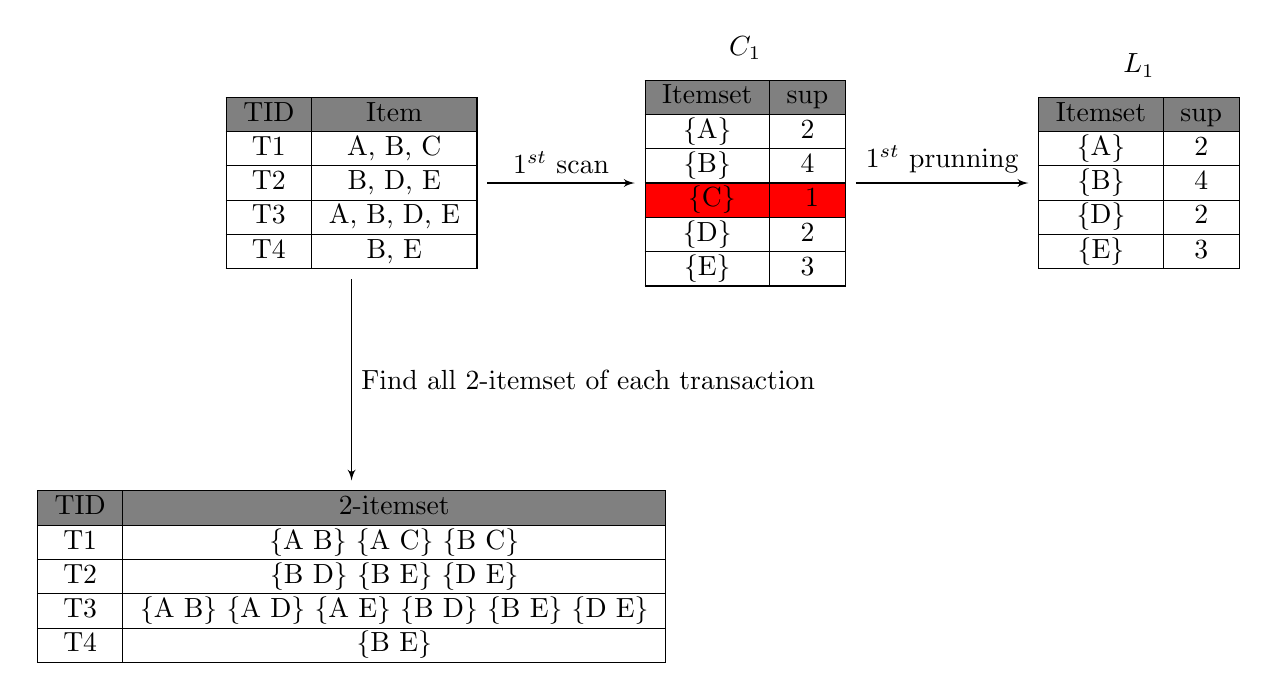
\begin{tikzpicture}[node distance = 5cm, auto]
  % Define block styles
  \tikzstyle{block} = [rectangle, fill=none,
                      text centered, rounded corners, minimum height=4em]
  \tikzstyle{line} = [draw, -latex']

  % Place nodes
  \node [block] (item1) {
    \begin{tabular}{|c|c|c|}
      \hline
        \rowcolor{Gray} % Set the color of the first row to gray
        TID & Item \\
        \hline
        T1 & A, B, C \\
        \hline
        T2 & B, D, E \\
        \hline
        T3 & A, B, D, E \\
        \hline
        T4 & B, E \\
        \hline
    \end{tabular}
  };

  \node [block, right of=item1, label=above:$C_1$] (scan1) {
    \begin{tabular}{|c|c|c|}
      \hline
        \rowcolor{Gray} % Set the color of the first row to gray
        Itemset & sup \\
        \hline
        {\{A\}} & 2 \\
        \hline
        {\{B\}} & 4 \\
        \hline
        \cellcolor{red} {\{C\}} & \cellcolor{red} 1 \\
        \hline
        {\{D\}} & 2 \\
        \hline
        {\{E\}} & 3 \\
        \hline
    \end{tabular}
  };

  \node [block, right of=scan1, label=above:$L_1$] (prunning1) {
    \begin{tabular}{|c|c|c|}
      \hline
        \rowcolor{Gray} % Set the color of the first row to gray
        Itemset & sup \\
        \hline
        {\{A\}} & 2 \\
        \hline
        {\{B\}} & 4 \\
        \hline
        {\{D\}} & 2 \\
        \hline
        {\{E\}} & 3 \\
        \hline
    \end{tabular}
  };

  \node [block, below of=item1] (2set) {
    \begin{tabular}{|c|c|c|}
      \hline
        \rowcolor{Gray} % Set the color of the first row to gray
        TID & 2-itemset \\
        \hline
        T1 & \{A B\} \{A C\} \{B C\} \\
        \hline
        T2 & \{B D\} \{B E\} \{D E\} \\
        \hline
        T3 & \{A B\} \{A D\} \{A E\} \{B D\} \{B E\} \{D E\} \\
        \hline
        T4 & \{B E\} \\
        \hline
    \end{tabular}
  };

  % Draw edges
  \path [line] (item1) -- (scan1) node[midway, above] {$1^{st}$ scan};
  \path [line] (scan1) -- (prunning1) node[midway, above] {$1^{st}$ prunning};
  \path [line] (item1) -- (2set) node[midway, right] {Find all 2-itemset of each transaction};

\end{tikzpicture}

Because we have:

\begin{itemize}
  \item Items = A, B, C, D, E,
  \item Order = 1, 2, 3, 4, 5
  \item Hash function : $h(\{x y\}) = (($order of $x)*10+($order of $y)) \% 7$
\end{itemize}

Thus we have the hash table below:

\begin{tabular}{|c|c|c|c|c|c|c|c|}
  \hline
    \rowcolor{Gray} % Set the color of the first row to gray
    bucket & 0 & 1 & 2 & 3 & 4 & 5 & 6 \\
    \hline
    count & 1 & 1 & 1 & 4 & 3 & 2 & 1 \\
    \hline
    2-itemset & \{A D\} & \{A E\} & \{B C\} & \{B D\} & \{B E\} & \{A B\} & \{A C\} \\
    &  &  &  & \{D E\} & \{B E\} & \{A B\} & \\
    &  &  &  & \{B D\} & \{B E\} &  &  \\
    &  &  &  & \{D E\} &  &  &  \\
    \hline
\end{tabular}

\newpage

Let $L_1$*$L_1$ to generate a 2-itemset table, and choose the itemsets where the number of content in its bucket is above the minimum support.

\begin{tikzpicture}[node distance = 5.5cm, auto]
  % Define block styles
  \tikzstyle{block} = [rectangle, fill=none,
                      text centered, rounded corners, minimum height=4em]
  \tikzstyle{line} = [draw, -latex']

  % Place nodes
  \node [block] (2set) {
    \begin{tabular}{|c|c|c|}
      \hline
        \rowcolor{Gray} % Set the color of the first row to gray
        $L_1$*$L_1$ & \# in the bucket \\
        \hline
        \{A B\} & 2 \\
        \hline
        \cellcolor{red} \{A D\} & \cellcolor{red} 1 \\
        \hline
        \cellcolor{red} \{A E\} & \cellcolor{red} 1 \\
        \hline
        \{B D\} & 4 \\
        \hline
        \{B E\} & 3 \\
        \hline
        \{D E\} & 4 \\
        \hline
    \end{tabular}
  };

  \node [block, right of=item1, label=above:$C_2$] (C2) {
    \begin{tabular}{|c|}
      \hline
        \rowcolor{Gray} % Set the color of the first row to gray
        Resulted $C_2$ \\
        \hline
        \{A B\} \\
        \hline
        \{B D\} \\
        \hline
        \{B E\} \\
        \hline
        \{D E\} \\
        \hline
    \end{tabular}
  };

  \node [block, right of=C2, label=above:$L_2$] (L2) {
    \begin{tabular}{|c|c|}
      \hline
        \rowcolor{Gray} % Set the color of the first row to gray
        $C_2$ & sup \\
        \hline
        \{A B\} & 2 \\
        \hline
        \{B D\} & 2 \\
        \hline
        \{B E\} & 3 \\
        \hline
        \{D E\} & 2 \\
        \hline
    \end{tabular}
  };

  % Draw edges
  \path [line] (2set) -- (C2) node[midway, above] {};
  \path [line] (C2) -- (L2);
\end{tikzpicture}

Because if an item occurs in a frequent ($k$+1)-itemset,
it must occur in at least k candidate k-itemsets.

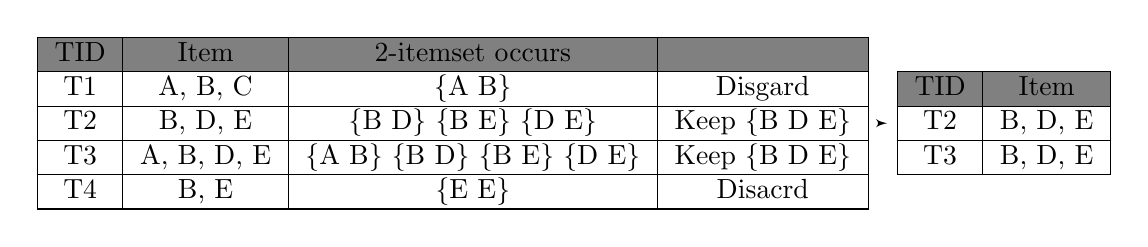
\begin{tikzpicture}[node distance = 7cm, auto]
  % Define block styles
  \tikzstyle{block} = [rectangle, fill=none,
                      text centered, rounded corners, minimum height=4em]
  \tikzstyle{line} = [draw, -latex']

  % Place nodes
  \node [block] (item1) {
    \begin{tabular}{|c|c|c|c|}
      \hline
      \rowcolor{Gray} % Set the color of the first row to gray
      TID & Item & 2-itemset occurs &  \\
      \hline
      T1 & A, B, C & \{A B\} & Disgard \\
      \hline
      T2 & B, D, E & \{B D\} \{B E\} \{D E\} & Keep \{B D E\} \\
      \hline
      T3 & A, B, D, E & \{A B\} \{B D\} \{B E\} \{D E\} & Keep \{B D E\}  \\
      \hline
      T4 & B, E & \{E E\} & Disacrd \\
      \hline
    \end{tabular}
  };

  \node [block, right of=item1] (item2) {
    \begin{tabular}{|c|c|c|}
      \hline
        \rowcolor{Gray} % Set the color of the first row to gray
        TID & Item \\
        \hline
        T2 & B, D, E \\
        \hline
        T3 & B, D, E \\
        \hline
    \end{tabular}
  };

  % Draw edges
  \path [line] (item1) -- (item2);
\end{tikzpicture}

Thus we have reduced the transactions.

\section*{Q3 [35 Marks]}

An itemset $X$ is said to be a frequent itemset if the frequency count of $X$ is at least a given support threshold.

An itemset $Y$ is a proper super-itemset of $X$ if $X \subset Y$ and $X \neq Y$. 

An itemset $X$ is said to be a closed frequent itemset 
if (1) $X$ is frequent 
and (2) there exists no proper super-itemset $Y$ of $X$ such that $Y$ is frequent 
and $Y$ has the same frequency count as $X$.

An itemset $X$ is said to be a maximal frequent itemset
if (1) $X$ is frequent
and (2) there exists no proper super-itemset $Y$ of $X$ such that $Y$ is frequent.

Let $F_c$ be the set of (traditional) frequent itemsets each of which is associated with a frequency in the dataset.

For example, if there are three frequent itemsets, \{$I_1$\} with frequency 4,
\{$I_2$\} with frequency 5, and \{$I_1, I_2$\} with frequency 3,
$F$=\{\{$I_1$\}, \{$I_2$\}, \{$I_2, I_2$\}\}
and $F_c = \{<\{I_1\}, 4>, <\{I_2\}, 5>, <\{I_1, I_2\}, 3>\}$.

Similarly, let $C$ be the set of closed frequent itemsets without specifying the frequency of itemsets.

Let $C_c$ be the set of closed frequent itemsets each of which is associated with a frequency of itemsets.

Let $M$ be the set of maximal frequent itemsets without specifying the frequency of itemsets.

Ler $M_c$ be the set of maximal frequent itemsets each of which is associated with a frequency in the dataset.

\newpage

The following shows six transactions with four items.
Each row corresponds to a transaction where 1 corresponds to a presence of an item and 0 corresponds to an absence.

\begin{tabular}{|c|c|c|c|}
  \hline
    \rowcolor{Gray} % Set the color of the first row to gray
    A & B & C & D \\
    \hline
    0 & 0 & 1 & 1 \\
    \hline
    1 & 1 & 0 & 0 \\
    \hline
    0 & 0 & 1 & 1 \\
    \hline
    1 & 0 & 1 & 1 \\
    \hline
    1 & 0 & 0 & 0 \\
    \hline
    0 & 0 & 0 & 1 \\
    \hline
\end{tabular}

Suppose that the support threshold is 2.

(a) (i) What is $F_C$? \hspace{1cm} (ii) What is $C_c$? \hspace{1cm} (iii)What is $M_c$? \textbf{(5 Marks)}

(b) (i) What is the advantages and the disadvantages of using closed frequent itemsets compared with traditional frequent itemsets? \textbf{(5 Marks)}

(ii) What are the advantages and the disadvantages of using closed frequent itemsets compared with maximal frequent itemsets? \textbf{(5 Marks)}

(c) Please adapt algorithm FP-growth with the use of the FP-tree to find all closed frequent item set.
Please write down how to adapt algorithm FP-growth and illustrate the adapted algorithm with the above example. \textbf{(20 Marks)}

\subsection*{Solution}

\paragraph*{(a)} According to the topic, we have the following transaction database. And we generate all the $k$-itemsets which might be frequent itemsets.

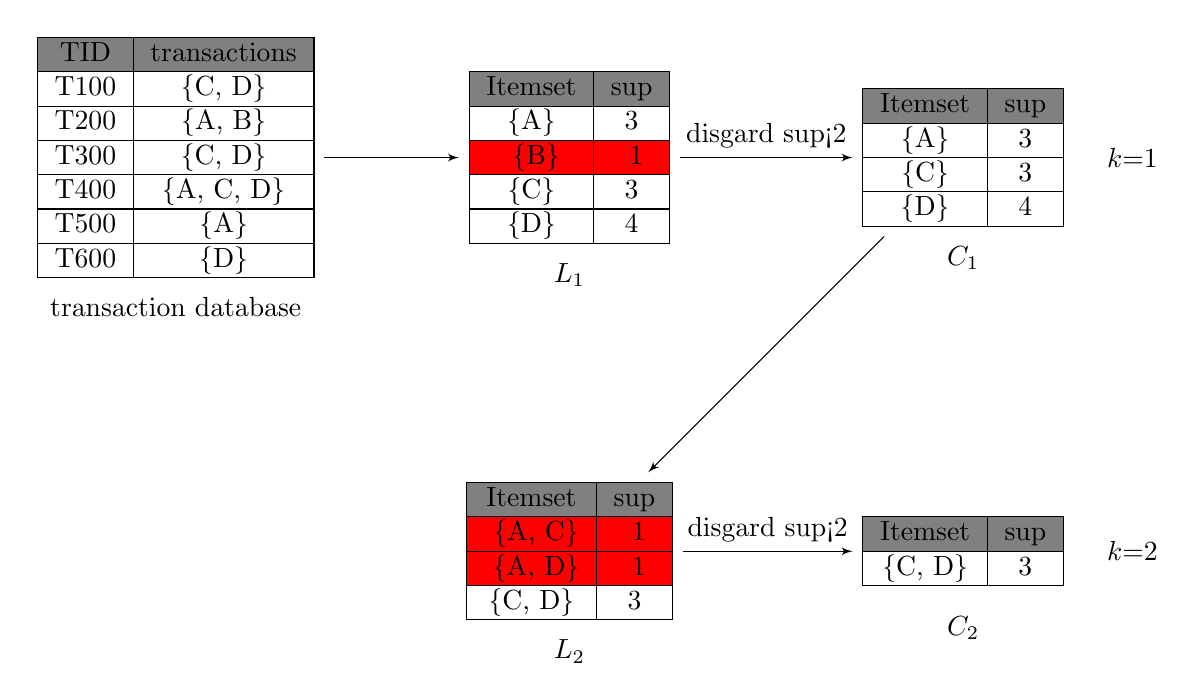
\begin{tikzpicture}[node distance = 5cm, auto]
  % Define block styles
  \tikzstyle{block} = [rectangle, fill=none,
                      text centered, rounded corners, minimum height=4em]
  \tikzstyle{line} = [draw, -latex']

  % Place nodes
  \node [block, label=below:{transaction database}] (DB) {
    \begin{tabular}{|c|c|}
      \hline
        \rowcolor{Gray} % Set the color of the first row to gray
        TID & transactions \\
        \hline
        T100 & \{C, D\} \\
        \hline
        T200 & \{A, B\} \\
        \hline
        T300 & \{C, D\} \\
        \hline
        T400 & \{A, C, D\} \\
        \hline
        T500 & \{A\} \\
        \hline
        T600 & \{D\} \\
        \hline
    \end{tabular}
  };

  \node [block, right of=DB, label=below:{$L_1$}] (L1) {
    \begin{tabular}{|c|c|}
      \hline
      \rowcolor{Gray} % Set the color of the first row to gray
      Itemset & sup  \\
      \hline
      \{A\} & 3 \\
      \hline
      \cellcolor{red} \{B\} & \cellcolor{red} 1 \\
      \hline
      \{C\} & 3  \\
      \hline
      \{D\} & 4 \\
      \hline
    \end{tabular}
  };

  \node [block, right of=L1, label=below:{$C_1$}] (C1) {
    \begin{tabular}{|c|c|}
      \hline
        \rowcolor{Gray} % Set the color of the first row to gray
        Itemset & sup \\
        \hline
        \{A\} & 3 \\
        \hline
        \{C\} & 3 \\
        \hline
        \{D\} & 4 \\
        \hline
    \end{tabular}
  };

  \node[left=of C1, xshift = 9cm] {$k$=1};

  \node [block, below of=L1, label=below:{$L_2$}] (L2) {
    \begin{tabular}{|c|c|}
      \hline
        \rowcolor{Gray} % Set the color of the first row to gray
        Itemset & sup \\
        \hline
        \cellcolor{red} \{A, C\} & \cellcolor{red} 1 \\
        \hline
        \cellcolor{red} \{A, D\} & \cellcolor{red} 1 \\
        \hline
        \{C, D\} & 3 \\
        \hline
    \end{tabular}
  };

  \node [block, right of=L2, label=below:{$C_2$}] (C2) {
    \begin{tabular}{|c|c|}
      \hline
        \rowcolor{Gray} % Set the color of the first row to gray
        Itemset & sup \\
        \hline
        \{C, D\} & 3 \\
        \hline
    \end{tabular}
  };

  \node[left=of C2, xshift = 9cm] {$k$=2};

  % Draw edges
  \path [line] (DB) -- (L1);
  \path [line] (L1) -- (C1) node [midway, above] {disgard sup<2};
  \path [line] (C1) -- (L2) node [midway, above] {};
  \path [line] (L2) -- (C2) node [midway, above] {disgard sup<2};
\end{tikzpicture}

\textbf{i}: We have $F_c = \{ <\{A\},3>, <\{C\},3>, <\{D\},4>, <\{C, D\},3>\}$

\textbf{ii}: We have $C_c = \{ <\{A\},3>, <\{D\},4>, <\{C, D\},3>\}$

\textbf{iii}: We have $M_c = \{ <\{A\},3>, <\{C, D\},3>\}$

\paragraph*{(b)} \textbf{i:}

\begin{itemize}
  \item Advantages: Compared with traditional frequent itemsets, inclosed itemsets are eliminated, which reduces the number of itemsets. And because a lot of frequent itemsets can be considered as subsets of a closed super-itemset, it does not lose much information.
  \item Disadvantages: Finding frequent closed itemsets need more computation, increasing the time complexity.
\end{itemize}

\textbf{ii:}

\begin{itemize}
  \item Advantages: Closed itemsets do not lose much information because the closed super-itemsets have same frequency as the sub-itemsets. But maximal frequent itemsets may lose some information.
  \item Disadvantages: Maximal frequent itemsets are more efficient than closed itemsets, because it does not need to check the frequency of the super-itemsets.
\end{itemize}

\paragraph*{(c)} 

Generate a FP-tree. Firstly, deduce the ordered frequent items.

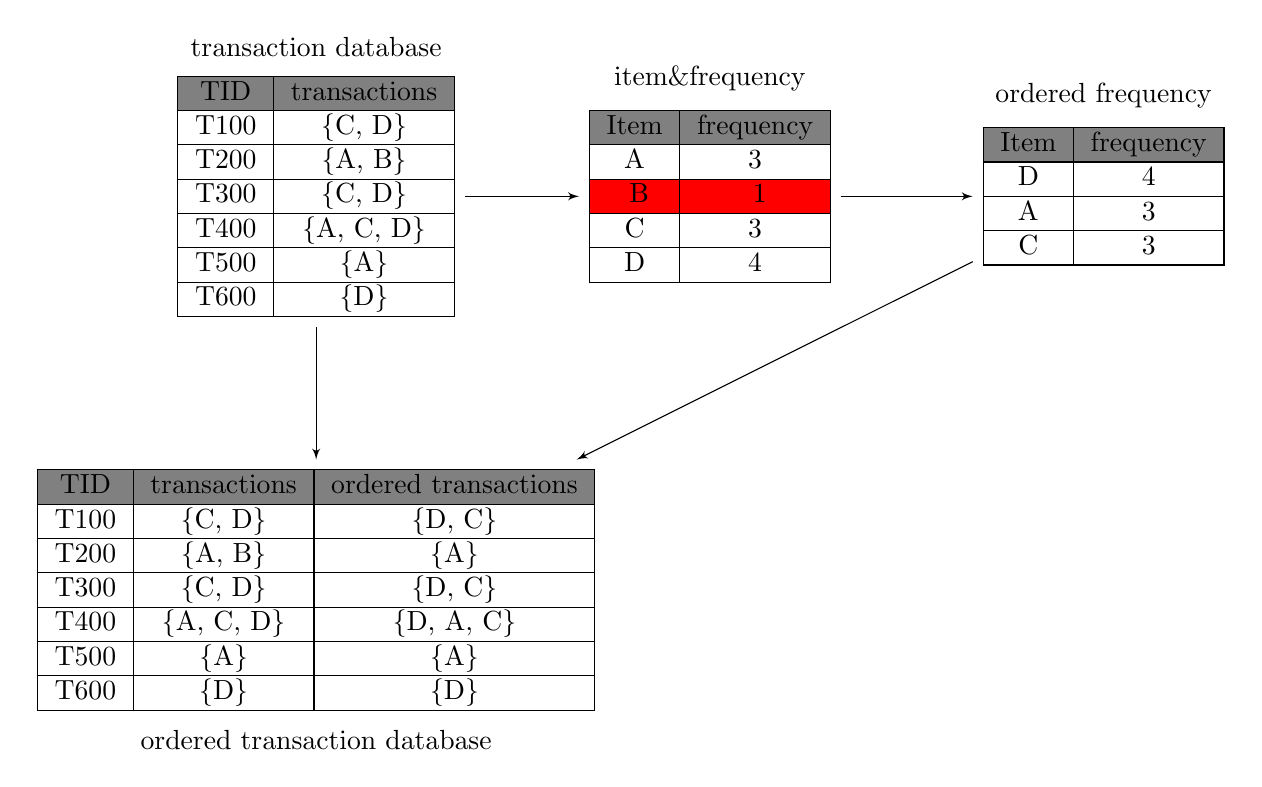
\begin{tikzpicture}[node distance = 5cm, auto]
  % Define block styles
  \tikzstyle{block} = [rectangle, fill=none,
                      text centered, rounded corners, minimum height=4em]
  \tikzstyle{line} = [draw, -latex']

    % Place nodes
    \node [block, label=above:{transaction database}] (DB) {
      \begin{tabular}{|c|c|}
        \hline
          \rowcolor{Gray} % Set the color of the first row to gray
          TID & transactions \\
          \hline
          T100 & \{C, D\} \\
          \hline
          T200 & \{A, B\} \\
          \hline
          T300 & \{C, D\} \\
          \hline
          T400 & \{A, C, D\} \\
          \hline
          T500 & \{A\} \\
          \hline
          T600 & \{D\} \\
          \hline
      \end{tabular}
    };

    \node [block, right of=DB, label=above:{item\&frequency}] (item) {
      \begin{tabular}{|c|c|}
        \hline
          \rowcolor{Gray} % Set the color of the first row to gray
          Item  & frequency \\
          \hline
          A & 3 \\
          \hline
          \cellcolor{red} B & \cellcolor{red} 1 \\
          \hline
          C & 3 \\
          \hline
          D & 4 \\
          \hline
      \end{tabular}
    };

    \node [block, right of=item, label=above:{ordered frequency}] (oitem) {
      \begin{tabular}{|c|c|}
        \hline
          \rowcolor{Gray} % Set the color of the first row to gray
          Item  & frequency \\
          \hline
          D & 4 \\
          \hline
          A & 3 \\
          \hline
          C & 3 \\
          \hline
      \end{tabular}
    };

    \node [block, below of=DB, label=below:{ordered transaction database}] (oDB) {
      \begin{tabular}{|c|c|c|}
        \hline
          \rowcolor{Gray} % Set the color of the first row to gray
          TID & transactions & ordered transactions\\
          \hline
          T100 & \{C, D\} & \{D, C\}\\
          \hline
          T200 & \{A, B\} & \{A\} \\
          \hline
          T300 & \{C, D\} & \{D, C\} \\
          \hline
          T400 & \{A, C, D\} & \{D, A, C\} \\
          \hline
          T500 & \{A\} & \{A\} \\
          \hline
          T600 & \{D\} & \{D\} \\
          \hline
      \end{tabular}
    };

  \path [line] (DB) -- (item);
  \path [line] (item) -- (oitem);
  \path [line] (oitem) -- (oDB);
  \path [line] (DB) -- (oDB);
\end{tikzpicture}

\newpage

Then we construct the FP-tree from the above data.

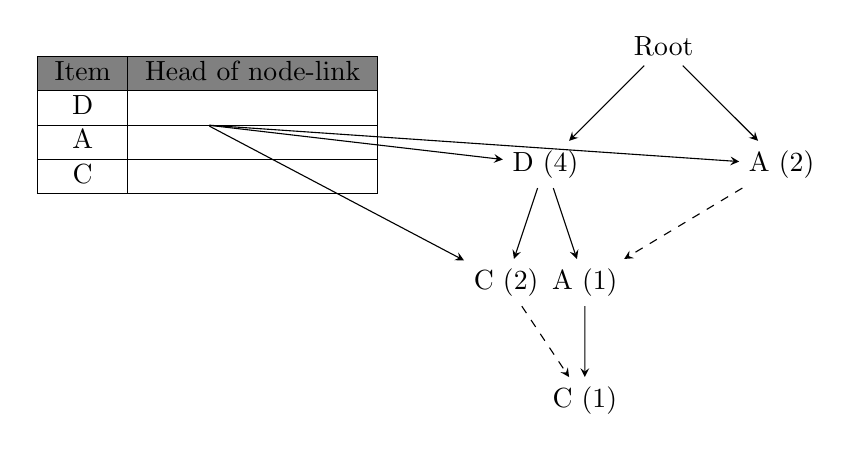
\begin{tikzpicture}[
  level 1/.style={sibling distance=3cm},
  level 2/.style={sibling distance=1cm}, 
  edge from parent/.style={->,draw},
  >=latex,
  >=stealth, remember picture]
  % Place the table using tabular inside a node
  \node (table) {
      \begin{tabular}{|c|c|}
        \hline
          \rowcolor{Gray} % Set the color of the first row to gray
          Item & Head of node-link \\
          \hline
          D & \tikz \node[inner sep=0pt] (celld) {}; \\
          \hline
          A & \tikz \node[inner sep=0pt] (cella) {}; \\
          \hline
          C & \tikz \node[inner sep=0pt] (cellc) {}; \\
          \hline
      \end{tabular}
  };

  % root of the tree
  \node [right=3cm of table, yshift = 1cm] {Root}
  % child 1
    child {node (D) {D (4)}
      child {node (C1) {C (2)}}
      child {node (A1) {A (1)}
        child {node (C2) {C (1)}}
      }
    }
  % child 2
    child {node (A2) {A (2)}};

  \draw [dashed, ->] (C1) -- (C2);
  \draw [dashed, ->] (A2) -- (A1);

  % Draw the arrow from the table cell to the tree node
  \draw[->] (celld) -- (D);
  \draw[->] (cella) -- (A2);
  \draw[->] (cellc) -- (C1);
\end{tikzpicture}

Construct the FP-conditional tree for $C, A, D$.

\textbf{for $C$}

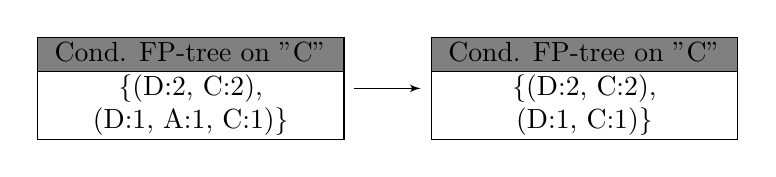
\begin{tikzpicture}[node distance = 5cm, auto]
  % Define block styles
  \tikzstyle{block} = [rectangle, fill=none,
                      text centered, rounded corners, minimum height=4em]
  \tikzstyle{line} = [draw, -latex']

    % Place nodes
    \node [block] (cFPC) {
      \begin{tabular}{|c|c|}
        \hline
          \rowcolor{Gray} % Set the color of the first row to gray
          Cond. FP-tree on "C" \\
          \hline
          \{(D:2, C:2), \\
          (D:1, A:1, C:1)\} \\
          \hline
      \end{tabular}
    };

    \node [block, right of=cFPC] (cPC) {
      \begin{tabular}{|c|c|}
        \hline
          \rowcolor{Gray} % Set the color of the first row to gray
          Cond. FP-tree on "C" \\
          \hline
          \{(D:2, C:2), \\
          (D:1, C:1)\} \\
          \hline
      \end{tabular}
    };

  \path [line] (cFPC) -- (cPC);
\end{tikzpicture}

Because for every path lying $C$, $D$ also lies in the path, so $C$ is not a closed frequent itemset. 
But $\{D, C\}$ is a closed frequent itemset.

\textbf{for $A$}

\begin{tikzpicture}[node distance = 5cm, auto]
  % Define block styles
  \tikzstyle{block} = [rectangle, fill=none,
                      text centered, rounded corners, minimum height=4em]
  \tikzstyle{line} = [draw, -latex']

    % Place nodes
    \node [block] (cFPA) {
      \begin{tabular}{|c|c|}
        \hline
          \rowcolor{Gray} % Set the color of the first row to gray
          Cond. FP-tree on "A" \\
          \hline
          \{(D:1, A:1), \\
          (A:2)\} \\
          \hline
      \end{tabular}
    };

    \node [block, right of=cFPC] (cPA) {
      \begin{tabular}{|c|c|}
        \hline
          \rowcolor{Gray} % Set the color of the first row to gray
          Cond. FP-tree on "A" \\
          \hline
          \{(A:3),\} \\
          \hline
      \end{tabular}
    };

  \path [line] (cFPA) -- (cPA);
\end{tikzpicture}

Because there is no other itemsets lies in the right path lying $A$, so $A$ is a closed frequent itemset.

\textbf{for $D$}

\begin{tikzpicture}[node distance = 5cm, auto]
  % Define block styles
  \tikzstyle{block} = [rectangle, fill=none,
                      text centered, rounded corners, minimum height=4em]
  \tikzstyle{line} = [draw, -latex']

    % Place nodes
    \node [block] (cFPD) {
      \begin{tabular}{|c|c|}
        \hline
          \rowcolor{Gray} % Set the color of the first row to gray
          Cond. FP-tree on "D" \\
          \hline
          \{(D:4)\} \\
          \hline
      \end{tabular}
    };

    \node [block, right of=cFPC] (cPD) {
      \begin{tabular}{|c|c|}
        \hline
          \rowcolor{Gray} % Set the color of the first row to gray
          Cond. FP-tree on "D" \\
          \hline
          \{(D:4),\}\\
          \hline
      \end{tabular}
    };

  \path [line] (cFPD) -- (cPD);
\end{tikzpicture}

Because there is a path only lying $D$, so $D$ is a closed frequent itemset.

Thus we have $C_c = \{ <\{D, C\},3>, <\{A\},3>, <\{D\},4>\}$. 

\newpage

\section*{Q4 [35 Marks]}

A GSP example: Suppose now we have 5 events: 'Upload Songs', 'Add Tags', 'Share', 'Listen' and 'Comment'.
Let min-support be 40\%.
The sequence database of a Music Platform is shown in following table:

\begin{tabular}{|c|c|}
  \hline
    \rowcolor{Gray} % Set the color of the first row to gray
    Object & Sequence \\
    \hline
    A & <\{'Upload Songs', 'Add Tags'\}> \\
    \hline
    B & <\{'Upload Songs', 'Share'\}> \\
    \hline
    C & <\{'Upload Songs'\}, \{'Share', 'Listen'\}> \\
    \hline
    D & <\{'Upload Songs'\}, \{'Upload Songs', 'Add Tags'\}, \{'Listen'\}> \\
    \hline
    E & <\{'Listen'\}, \{'Add Tags', 'Comment'\}, \{'Share', 'Listen'\}> \\
    \hline
\end{tabular}

Please answer the following questions:

(a) Make the first pass over the sequence database to yield all the 1-element \textbf{frequent} sequences and what is the corresponding support? \textbf{5 Marks}

(b) Based on (a), do the 2-sequences Candidate Generation and Candidate Pruning. \textbf{10 Marks}

(c) What is the \textbf{frequent} 2-sequences based on the result of (b)? \textbf{5 Marks}

(d) Based on (c), do the 3-sequences Candidate Generation and Candidate Pruning.
When a sequence should be pruned, you need to explain why. \textbf{10 Marks}

(e) What is the frequent 3-sequences based on the result of (d)?
Please calculate the support. \textbf{5 Marks}

\textbf{Remember: For frequent k-sequences, the support >= min-support}

\subsection*{Solution}

For easier reading, we denote 'Upload Songs', 'Add Tags', 'Share', 'Listen' and 'Comment' by U, A, S, L and C respectively.
And if there are 2 items in 1 set, we have arranged it in alphabetical order by the first letter.
Thus we have:

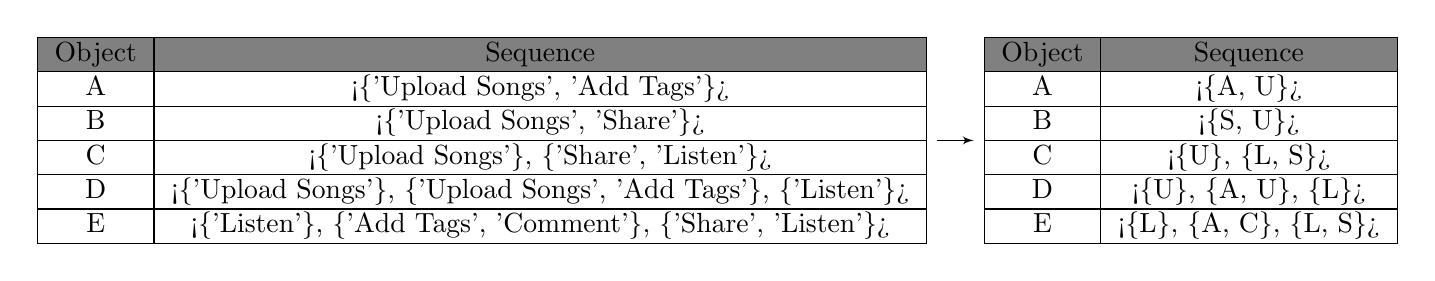
\begin{tikzpicture}[node distance = 9cm, auto]
  % Define block styles
  \tikzstyle{block} = [rectangle, fill=none,
                      text centered, rounded corners, minimum height=4em]
  \tikzstyle{line} = [draw, -latex']

    % Place nodes
    \node [block] (DB) {
      \begin{tabular}{|c|c|}
        \hline
          \rowcolor{Gray} % Set the color of the first row to gray
          Object & Sequence \\
          \hline
          A & <\{'Upload Songs', 'Add Tags'\}> \\
          \hline
          B & <\{'Upload Songs', 'Share'\}> \\
          \hline
          C & <\{'Upload Songs'\}, \{'Share', 'Listen'\}> \\
          \hline
          D & <\{'Upload Songs'\}, \{'Upload Songs', 'Add Tags'\}, \{'Listen'\}> \\
          \hline
          E & <\{'Listen'\}, \{'Add Tags', 'Comment'\}, \{'Share', 'Listen'\}> \\
          \hline
      \end{tabular}
    };

    \node [block, right of=DB] (tDB) {
        \begin{tabular}{|c|c|}
          \hline
            \rowcolor{Gray} % Set the color of the first row to gray
            Object & Sequence \\
            \hline
            A & <\{A, U\}> \\
            \hline
            B & <\{S, U\}> \\
            \hline
            C & <\{U\}, \{L, S\}> \\
            \hline
            D & <\{U\}, \{A, U\}, \{L\}> \\
            \hline
            E & <\{L\}, \{A, C\}, \{L, S\}> \\
            \hline
        \end{tabular}
    };

    \path [line] (DB) -- (tDB);
\end{tikzpicture}

\paragraph*{(a)} Candidate 1-sequences are:

<\{A\}>, <\{C\}>, <\{L\}>, <\{S\}>, <\{U\}>

\newpage

According to the database above, we have:

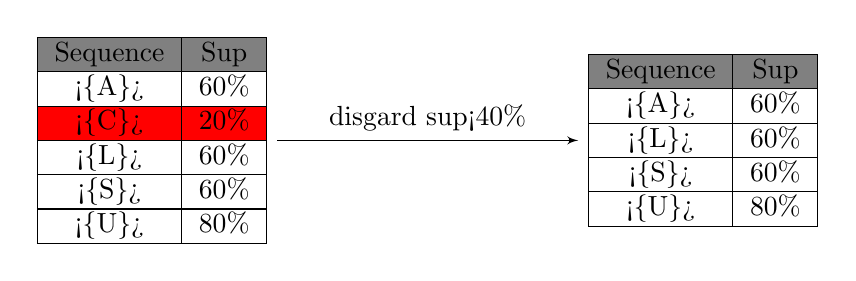
\begin{tikzpicture}[node distance = 7cm, auto]
  % Define block styles
  \tikzstyle{block} = [rectangle, fill=none,
                      text centered, rounded corners, minimum height=4em]
  \tikzstyle{line} = [draw, -latex']

    % Place nodes
    \node [block] (C1) {
      \begin{tabular}{|c|c|}
        \hline
          \rowcolor{Gray} % Set the color of the first row to gray
          Sequence & Sup \\
          \hline
          <\{A\}> & 60\% \\
          \hline
          \cellcolor{red}<\{C\}> & \cellcolor{red}20\% \\
          \hline
          <\{L\}> & 60\% \\
          \hline
          <\{S\}> & 60\% \\
          \hline
          <\{U\}> & 80\% \\
          \hline
      \end{tabular}
    };

    \node [block, right of=C1] (L1) {
        \begin{tabular}{|c|c|}
          \hline
            \rowcolor{Gray} % Set the color of the first row to gray
            Sequence & Sup \\
            \hline
            <\{A\}> & 60\% \\
            \hline
            <\{L\}> & 60\% \\
            \hline
            <\{S\}> & 60\% \\
            \hline
            <\{U\}> & 80\% \\
            \hline
        \end{tabular}
    };

    \path [line] (C1) -- (L1) node [midway, above] {disgard sup<40\%};
\end{tikzpicture}

The 1-element frequent sequences and the corresponding support are:

<\{'Add Tags'\}> (support=60\%)

<\{'Listen'\}> (support=60\%)

<\{'Share'\}> (support=60\%)

<\{'Upload Songs'\}> (support=80\%)

\paragraph*{(b)}

Base case $(k=2)$: Merging two frequent 1-sequences <\{$i_1$\}> and <\{$i_2$\}> will produce two candidate 2-sequences: <\{$i_1$\} \{$i_2$\}> and <\{$i_1 , i_2$\}>

Candidate 2-sequences are:

<\{A, L\}>, <\{A, S\}>, <\{A, U\}>, <\{L, S\}>, <\{L, U\}>, <\{S, U\}>,

<\{A\}, \{A\}>, <\{A\}, \{L\}>, <\{A\}, \{S\}>, <\{A\}, \{U\}>, 

<\{L\}, \{A\}>, <\{L\}, \{L\}>, <\{L\}, \{S\}>, <\{L\}, \{U\}>, 

<\{S\}, \{A\}>, <\{S\}, \{L\}>, <\{S\}, \{S\}>, <\{S\}, \{U\}>, 

<\{U\}, \{A\}>, <\{U\}, \{L\}>, <\{U\}, \{S\}>, <\{U\}, \{U\}>

All the 1-sequences we generate 2-sequences from are frequent. So after candidate prunning, the 2-sequences should remain the same.

\paragraph*{(c)}

After candidate elimination, frequent 2-sequences are:

<\{A, U\}> (support=40\%),

<\{L, S\}> (support=40\%),

<\{A\}, \{L\}> (support=40\%),

<\{U\}, \{L\}> (support=40\%)

\paragraph*{(d)}

Generate 3-sequences from the remaining 2-sequences, 3-sequences are:

<\{A, U\}, \{L\}> (generate from <\{A, U\}> and <\{U\}, \{L\}> or from <\{A, U\}> and <\{A\}, \{L\}> ),

<\{A\}, \{L, S\}> (generate from <\{A\}, \{L\}> and <\{L, S\}),

<\{U\}, \{L, S\}> (generate from <\{U\}, \{L\}> and <\{L, S\})

Pruning:

<\{A\}, \{L, S\}> should be pruned because one 2-subsequence <\{A\}, \{S\}> is not frequent.

<\{U\}, \{L, S\}> should be pruned because one 2-subsequence <\{U\}, \{S\}> is not frequent.

\paragraph*{(e)}

<\{A, U\}, \{L\}> (support=20\% < 40\%, should be eliminated)

Thus, there is no frequent 3-sequence.

\end{document}
